\section{Χωρικός Κατακερματισμός Πολλαπλής Ανάλυσης}
\label{section4:NeuralHashGridEncoding}
\par
    Η διαδικασία \enit{multi-resolution hash encoding} όπως είπαμε αφορά την κωδικοποίηση του δικτύου με βάση την διαμέριση του χώρου.
\par 
    Ο τρόπος που εφαρμόζεται κάτι τέτοιο είναι με το σπάσιμο του χώρου σε μερικά πλέγματα (\enit{Grids}) τετραγώνων εφόσον το πεδίο που εφαρμόζεται ας πούμε είναι εικόνες τα οποία θα αυξάνουν σε ανάλυση. Αυτό θα εφαρμόζεται ιεραρχικά και μπορεί να οριστεί όμως σε οποιοδήποτε χώρο δεδομένων (παραδείγματος χάρη μπορεί να εφαρμοστεί στο NeRF που χρησιμοποιεί μαζί το σημείο της εικόνας με το τρισδιάστατο διάνυσμα της ακτίνας που περνά από το pixel).
\par
    Έστω πως \textbf{d} είναι οι διαστάσεις της εισόδου. Η ανάλυση του κάθε πλέγματος διαμέρισης είναι σταθερή και διαφορετική από το προηγούμενο επίπεδο διαμέρισης αλλά δεν χρειάζεται ο τρόπος με τον οποίο ανεβάζουμε την ανάλυση διαμέρισης να είναι σταθερός. Έτσι διακρίνονται οι παρακάτω υπερπαράμετροι αυτής της μεθοδολογίας:
    \begin{itemize}
        \item  $ L $ := Πλήθος Επιπέδων Ανάλυσης 
        \item  $N_{min}$ := Ελάχιστη Ανάλυση πλέγματος
        \item  $N_{max}$ := Μέγιστη Ανάλυση πλέγματος
    \end{itemize}
    και ο τρόπος υπολογισμού του παράγοντα αύξησης ανάλυσης να δίνεται από τον τύπο (γεωμετρική πρόοδος μεταξύ χαμηλής και υψηλής ανάλυσης ογκομετρικού πλέγματος \enit{grid})
    \[ b := \exp{\frac{\ln{N_{max}} - \ln{N_{min}}}{L  - 1}}\]
    Συνεπώς η ανάλυση του πλέγματος σε ένα επίπεδο $\ell$ είναι $N_{\ell}:=\left\lfloor N_{\min }\cdot b^{\ell}\right\rfloor$

\par 
    Ο μετασχηματισμός της εισόδου σε κάποια επιλεγμένη ανάλυση γίνεται πρώτα κλιμακώνοντας το ζητούμενο σημείο $x$ κατά την ανάλυση του \enit{grid}, $N_{\ell}$ και εφαρμόζοντας στρογγυλοποίηση προς τα πάνω ή κάτω για να βρούμε το κελί που έχει το x. Αυτό το κελί αποτελεί τη χωρική θέση του σημείου στο grid.

\par 
    Αφού βρεθεί η θέση για να αποδοθεί το χαρακτηριστικό των συντεταγμένων εφαρμόζεται μετασχηματισμός κατακερματισμού  \enit{Hash Encoding}. Όπου εισάγονται άλλες δύο υπερπαράμετροι που καθορίζουν και την αναλυτικότητα κωδικοποίησης:
    \begin{itemize}
        \item $T := $ Μέγεθος Πίνακα Κατακερματισμού, 
        \item $F := $ Μέγιστος αριθμός χαρακτηριστικών συντεταγμένων ανά κελί, 
    \end{itemize}

    με την συνάρτηση κατακερματισμού να είναι μια συνάρτηση που εφαρμόζει \enit{bitwise XOR}, όπως αναφέρθηκε και στο θεωρητικό υπόβαθρο και η εφαρμογή του \enit{hash} χαρακτηριστικού στον πίνακα να γίνεται απλά εφαρμόζοντας την πράξη της ακέραιας διαίρεσης του \enit{hash} με τον μέγεθος του  πίνακα $T$
    \begin{equation}
        h(\mathbf{x})=\bigoplus_{i=1}^d x_i \pi_i  \mod T
        \label{hashfunction}
    \end{equation}

    Κάθε κελί έχει $F$ παραμέτρους εκπαίδευσης.
    Κατά την διάρκεια της εκπαίδευσης γίνεται οπισθοδιάδοση των κλίσεων μέχρι και τους πίνακες \enit{hash} ώστε να δυναμικά να εκπαιδευτεί η κωδικοποίηση και αυτή η χωρική διαμέριση. Όπως αναφέρθηκε δεν γίνεται χειρισμός των \enit{hash} συμπίπτουν (λόγω φύσης της συνάρτησης κατακερματισμού), αλλά κατά την διάρκεια της εκπαίδευσης γίνονται τα χαρακτηριστικά \enit{hash} ανθεκτικά σε αυτό το φαινόμενο, που υπό βοηθείται και από τους παραμέτρους \enit{$\pi_i$} που βελτιώνουν την συνοχή προσωρινής μνήμης αλλά σε μικρή κλίμακα δεν λύνει το πρόβλημα. 
\par
    Τρίτο βήμα σε αυτή την διαδικασία αποτελεί η παλινδρόμηση η οποία αφορά την γραμμική προσέγγιση των $2^d$ πινάκων \enit{hash} που αντιστοιχούν στο παρόν κελί του πλέγματος. Αυτή η διαδικασία πραγματοποιείται είτε με δι-γραμμική παρεμβολή σε δύο διαστάσεις είτε με τριγραμμική. Δηλαδή στις δύο διαστάσεις με δυο οριζόντιες παρεμβολές στις τετμημένες πρώτα και μετά στις τεταγμένες.Σε αυτό το σημείο εφαρμόζεται και το νευρωνικό στρώμα προσοχής το οποίο δεν διακριτοποιεί την συνάρτηση παλινδρόμησης άλλα αντιστοιχεί τις διακριτές τιμές των πινάκων σε βάρη τα οποία βελτιώνονται κατά την διαδικασία της εκπαίδευσης με τον αλγόριθμο βελτιστοποίησης (π.χ. Adam). Συνεπώς επί του συνόλου το \enit{hash encoding} αποτελεί συνεχή μορφή κωδικοποίησης παρ' όλη την διακριτή μορφή ορισμένων διαδικασιών που χρησιμοποιεί.

\par
    Τελευταίο βήμα αυτής της διαδικασίας είναι η συνένωση των χαρακτηριστικών διανυσμάτων που αντιστοιχήθηκε η είσοδος δημιουργώντας ένα συνολικό διάνυσμα διάστασης $L*F$ εφόσον έχουμε L πλήθος αναλύσεις F χαρακτηριστικών σημείων ανά ανάλυση. Τα οποία συνενώνονται με την ίδια την είσοδο δίνοντας μια ικανοποιητική μορφή πεδίου για το \enit{IDR}.
    
    Παρακάτω φαίνεται η αναπαράσταση του δικτύου μετασχηματισμού με είσοδο δύο διαστάσεων όπως περιγράφεται και τριών διαστάσεων, όπως αυτή που υλοποιήθηκε υλοποιήθηκε:

    \begin{figure}[H]
        \centering
        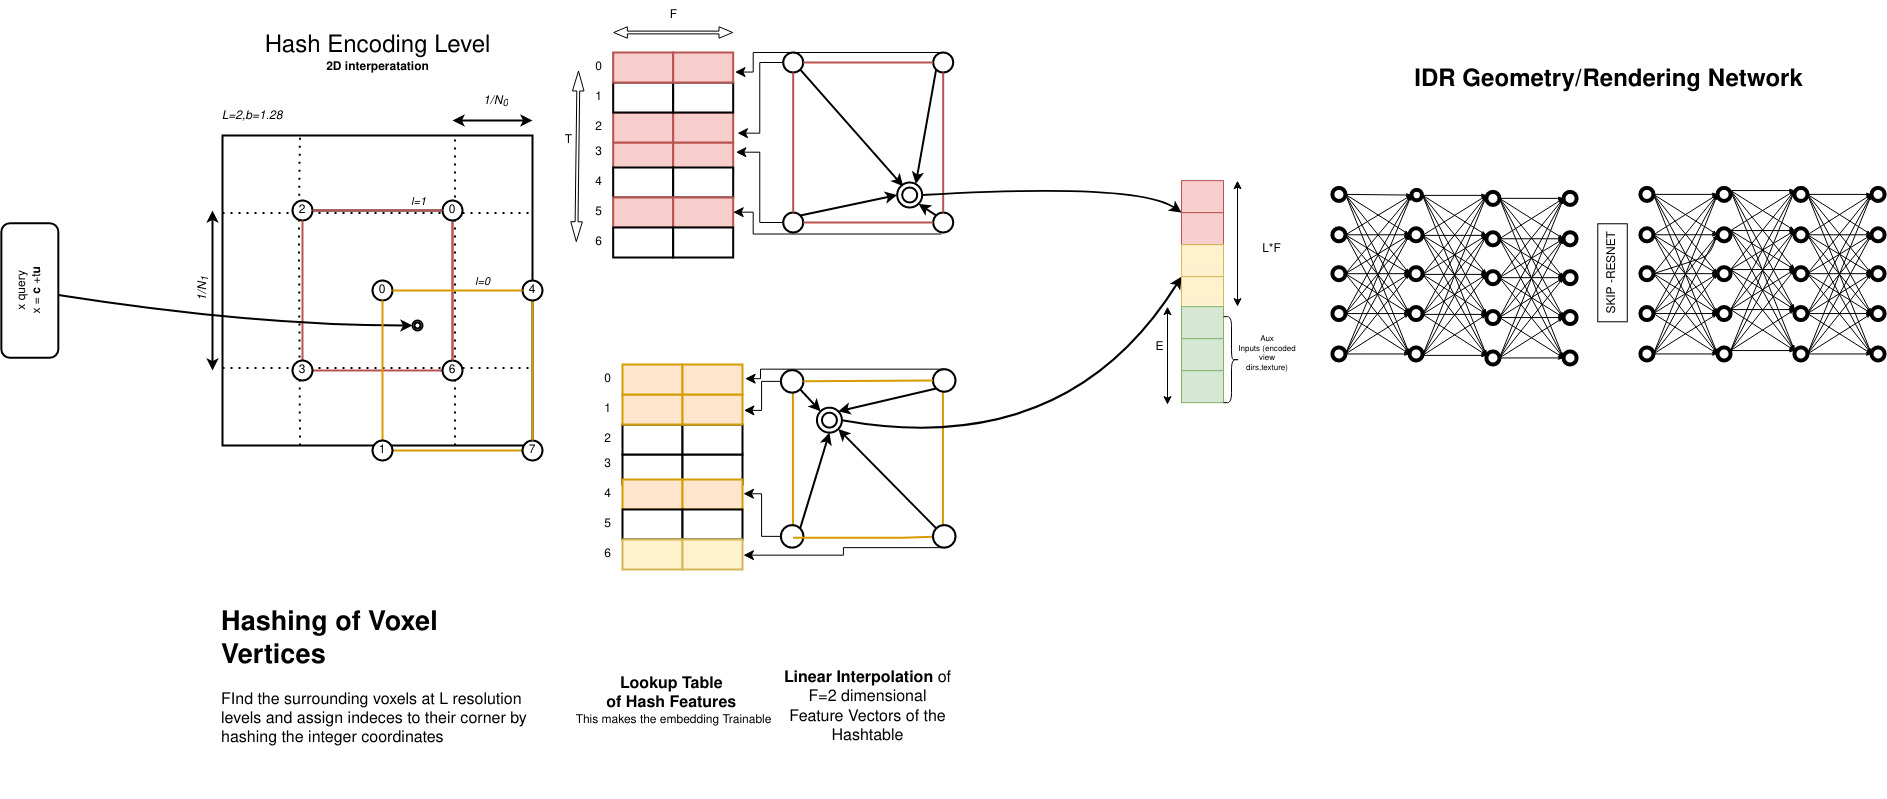
\includegraphics[width = \linewidth]{images/chapter4_img/IDR_Embeddings_Architecture-2D Hasgrid Encoding Net.drawio.jpg}
        \caption{2D ανάλογο end-to-end αρχιτεκτονικής δικτύου με χρήση Multi Resolution Hash Grid Encoding }
        \label{fig:2dhashgrid}
    \end{figure}
    
    \begin{figure}[H]
        \centering
        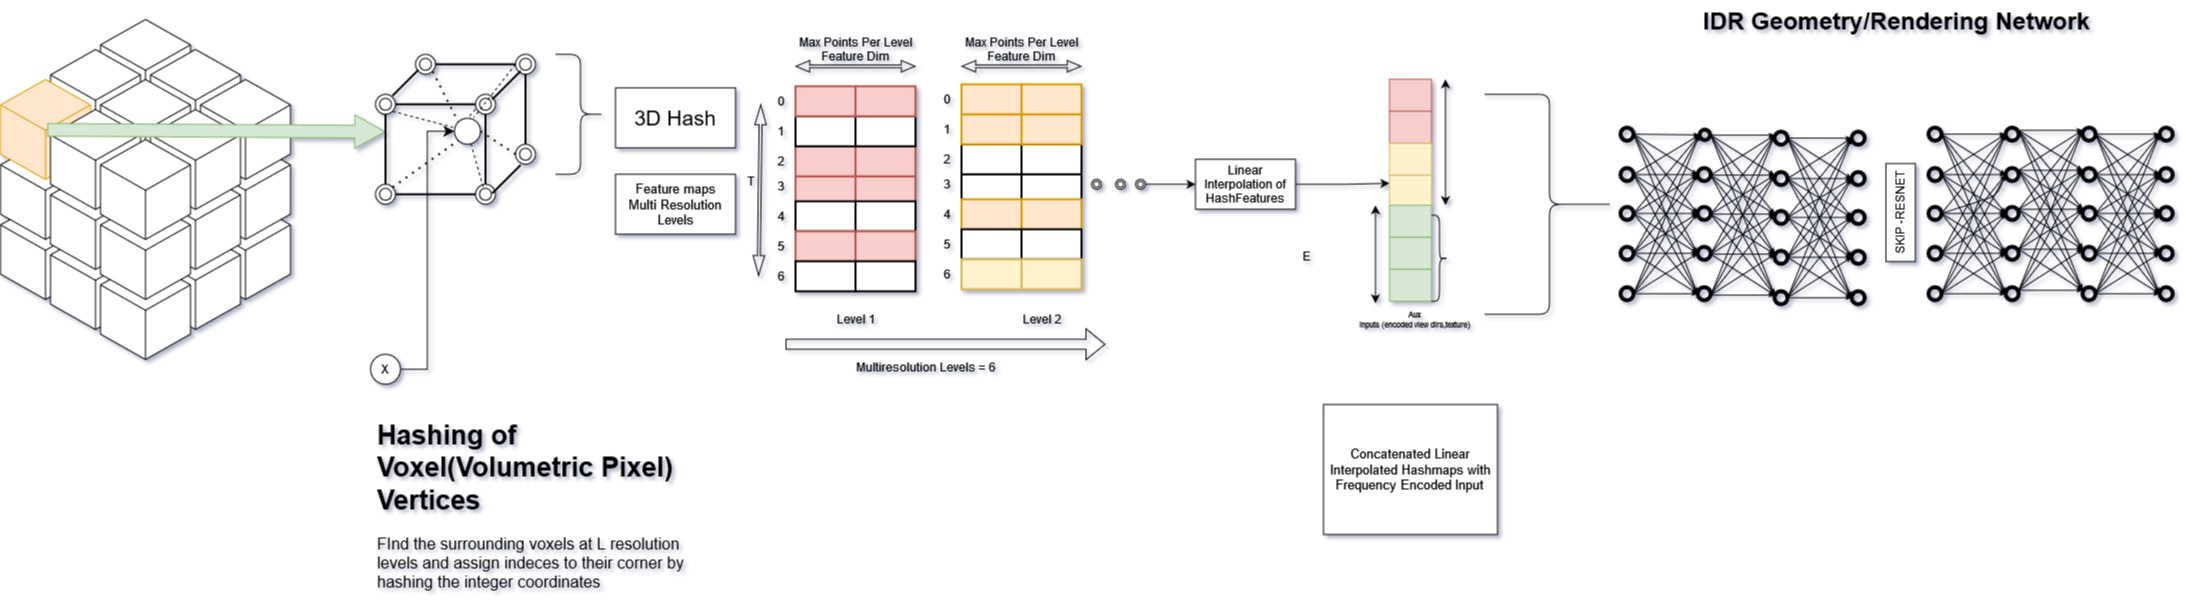
\includegraphics[width = \linewidth]{images/chapter4_img/IDR_Embeddings_Architecture-3D Hashgrid Embedding Net Equivalent.jpg}
        \caption{3D Hashgrid MLP IDR Proxy}
        \label{fig:hasgridmlp}
    \end{figure}

\par
    Στο Παράρτημα Γ \ref{section:appendix-algorithms}, υπάρχει μια πιο αναλυτική μορφή του αλγορίθμου που υλοποιήθηκε σε \enit{python} σε μορφή ψευδογλώσσας.
